% ---------- Titelblad Masterproef Faculteit Wetenschappen -----------
% Dit document is opgesteld voor compilatie met pdflatex.  Indien je
% wilt compileren met latex naar dvi/ps, dien je de figuren naar
% (e)ps-formaat om te zetten.
%                           -- december 2012
% -------------------------------------------------------------------
\RequirePackage{fix-cm}
\documentclass[12pt,a4paper,oneside]{book}

% --------------------- In te laden pakketten -----------------------
% Deze kan je eventueel toevoegen aan de pakketten die je al inlaadt
% als je dit titelblad integreert met de rest van thesis.
% -------------------------------------------------------------------
\usepackage{graphicx,xcolor,textpos}
\usepackage{helvet}
\usepackage[linktoc=all]{hyperref}
\usepackage[dutch]{babel}


% -------------------- Pagina-instellingen --------------------------
% Indien je deze wijzigt, zal het titelblad ook wijzigen.  Dit dien je
% dan manueel aan te passen.
% --------------------------------------------------------------------

\topmargin -10mm
\textwidth 160truemm
\textheight 240truemm
\oddsidemargin 0mm
\evensidemargin 0mm

% ------------------- textpos-instellingen ---------------------------
% Enkele andere instellingen voor het voorblad.
% --------------------------------------------------------------------

\definecolor{green}{RGB}{172,196,0}
\definecolor{bluetitle}{RGB}{29,141,176}
\definecolor{blueaff}{RGB}{0,0,128}
\definecolor{blueline}{RGB}{82,189,236}
\setlength{\TPHorizModule}{1mm}
\setlength{\TPVertModule}{1mm}

\begin{document}

% ---------------------- Voorblad ------------------------------------
% Vergeet niet de tekst aan te passen:
% - Titel en, indien van toepassing, ondertitel
%          voor eventuele formules in de titel of ondertitel
%          gebruik je  \form{$...$}
% - Je naam
% - Je (co)promotor, begeleider (indien van toepassing)
% - Je opleiding
% - Het academiejaar
% --------------------------------------------------------------------
\thispagestyle{empty}
\newcommand{\form}[1]{\scalebox{1.087}{\boldmath{#1}}}
\sffamily
%
\begin{textblock}{191}(-24,-11)
\colorbox{green}{\hspace{123mm}\ \parbox[c][18truemm]{68mm}{\textcolor{white}{FACULTEIT WETENSCHAPPEN}}}
\end{textblock}
%
\begin{textblock}{70}(-18,-19)
\textblockcolour{}
\includegraphics*[height=19.8truemm]{LogoKULeuven}
\end{textblock}
%
\begin{textblock}{160}(-6,63)
\textblockcolour{}
\vspace{-\parskip}
\flushleft
\fontsize{40}{42}\selectfont \textcolor{bluetitle}{Programmeren met kansen: Case study}\\[1.5mm]
%\fontsize{20}{22}\selectfont Ondertitel \form{$S=\pi r^2$\textsl{(facultatief)}}
\end{textblock}
%
\begin{textblock}{160}(8,153)
\textblockcolour{}
\vspace{-\parskip}
\flushright
\fontsize{14}{16}\selectfont \textbf{Sus VERWIMP}
\end{textblock}
%
\begin{textblock}{70}(-6,191)
\textblockcolour{}
\vspace{-\parskip}
\flushleft
Promotor: Prof. T. Schrijvers\\[-2pt]
\textcolor{blueaff}{Affiliatie \textsl{(facultatief)}}\\[5pt]
%Co-promotor: \textsl{(facultatief)}\\[-2pt]
%\textcolor{blueaff}{Affiliatie \textsl{(facultatief)}}\\[5pt]
Begeleider: \textsl{A. Vandenbroucke (facultatief)}\\[-2pt]
\textcolor{blueaff}{Affiliatie \textsl{(facultatief)}}\\
\end{textblock}
%
\begin{textblock}{160}(8,191)
\textblockcolour{}
\vspace{-\parskip}
\flushright
Proefschrift ingediend tot het\\[4.5pt]
behalen van de graad van\\[4.5pt]
Master of Science in\\[4.5pt]
Toegepaste Informatica\\
\end{textblock}
%
\begin{textblock}{160}(8,232)
\textblockcolour{}
\vspace{-\parskip}
\flushright
Academiejaar 2017-2018
\end{textblock}
%
\begin{textblock}{191}(-24,248)
{\color{blueline}\rule{550pt}{5.5pt}}
\end{textblock}
%
\vfill
\newpage

% Copyright statement
\textsf{\textcopyright} Copyright by KU Leuven
Zonder voorafgaande schriftelijke toestemming van zowel de promotor(en) als de auteur(s) is overnemen, kopiëren, gebruiken of realiseren van deze uitgave of gedeelten ervan verboden. Voor aanvragen tot of informatie i.v.m. het overnemen en/of gebruik en/of realisatie van gedeelten uit deze publicatie, wend u tot de KU Leuven, Faculteit Wetenschappen, Geel Huis, Kasteelpark Arenberg 11 bus 2100, 3001 Leuven (Heverlee), Telefoon +32 16 32 14 01.

Voorafgaande schriftelijke toestemming van de promotor(en) is eveneens vereist voor het aanwenden van de in dit afstudeerwerk beschreven (originele) methoden, producten, schakelingen en programma’s voor industrieel of commercieel nut en voor de inzending van deze publicatie ter deelname aan wetenschappelijke prijzen of wedstrijden.

\vfill
\newpage

% Als je het titelblad wil integreren met de rest van je thesis,
% kan je hieronder verder.
% ----------------------- Eerste pagina's -------------------------
% Hier kan je inhoudsopgave, voorwoord en dergelijke kwijt.
% -----------------------------------------------------------------
\rmfamily
\setcounter{page}{0}
\pagenumbering{roman}
\frontmatter
\chapter{Voorwoord}
\chapter{Korte Samenvatting}
\chapter{Lijst van afkortingen en lijst van symbolen}
\tableofcontents


\newpage
% ----------------------- Eigenlijke thesis -----------------------
% Vanaf de inleiding/het eerste hoofdstuk.
% -----------------------------------------------------------------
\mainmatter
\setcounter{page}{0}
\pagenumbering{arabic}
\chapter{Inleiding}
\chapter{Probabilistic Programming Languages}
Probabilistic Programming Languages of PPL's zijn programmeertalen die het modelleren van een onzekerheidsprobleem makkelijker maakt, en vragen over deze onzekerheden kunnen oplossen aan de hand van een inferentie methode. In hoofdstukken~\ref{sec:problog} en~\ref{sec:anglican} vindt u meer informatie over de implementatie en inferentie methodes van de twee PPL's die ik bespreek in deze thesis: Problog en Anglican.
\section{ProbLog}
\label{sec:problog}
\section{Anglican}
\label{sec:anglican}

\chapter{Stappenplan}
Om de twee PPL's te evalueren en vergelijken maak ik gebruik van een zelf verzonnen spel dat probabilistische aspecten bevat. Dit spel modelleer ik in ProbLog en Anglican. Na de implementatie kan ik beginnen met het vergelijken en evalueren van de PPL's aan de hand van verschillende kwalitatieve en kwantitatieve criteria.
\section{Spel}
Het spel bestaat uit een bord van 10 op 10 blokken. Elke blok in het bord heeft 1 toegewezen kleur. Er zijn 4 kleuren die aan een blok kunnen toegewezen worden: rood, groen, geel, blauw.\\\\
Elke beurt kan de speler op 1 van de blokken drukken. Als er op een blok wordt gedrukt, verandert deze van kleur. De kleur waar de blok in verandert hangt af van welke kleur de blok had voor dat er op gedrukt werd.
\begin{itemize}
  \item Een rode blok verandert met 1/3 kans in een groene blok, 1/3 kans in een blauwe blok en 1/3 kans in een gele blok.
  \item Een groene blok verandert met 1/3 kans in een rode blok, 1/3 kans in een blauwe blok en 1/3 kans in een gele blok.
  \item Een blauwe blok verandert met 1/3 kans in een rode blok, 1/3 kans in een groene blok en 1/3 kans in een gele blok.
  \item Een gele blok verandert met 1/3 kans in een rode blok, 1/3 kans in een groene blok en 1/3 kans in een blauwe blok.
\end{itemize}
\begin{figure}
  \centering
    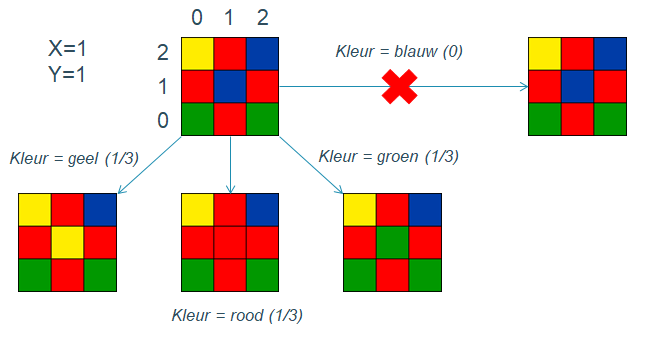
\includegraphics[height=55truemm]{game_change_blocks}
  \caption{In de figuur gebruik ik een 3x3 bord, als er op de middelste blauwe blok (1,1) wordt gedrukt, verandert de blok met 1/3 kans in een rode blok, met 1/3 kans in een groene en met 1/3 kans in een gele blok. De blauwe blok zal nooit in een blauwe blok veranderen. }
  \label{fig:game_change_blocks}
\end{figure}
Figuur~\ref{fig:game_change_blocks} geeft een visuele weergave van wat er gebeurd als er op een blok wordt gedrukt.\\\\
Als er drie of meer blokken van dezelfde kleur horizontaal/verticaal naast elkaar liggen verdwijnen ze en dit levert punten op. De blokken die zich boven de verdwenen blokken bevinden vallen naar beneden tot ze op een andere blok belanden ofwel op de bodem van het spelbord. De bedoeling van het spel is om in tien beurten zoveel mogelijk punten te behalen waarin de speler in elke beurt \'{e}\'{e}n blok van kleur kan veranderen. De beurt eindigt wanneer er geen 3 blokken van dezelfde kleur meer horizontaal en/of verticaal naast elkaar staan.
\begin{figure}
  \centering
    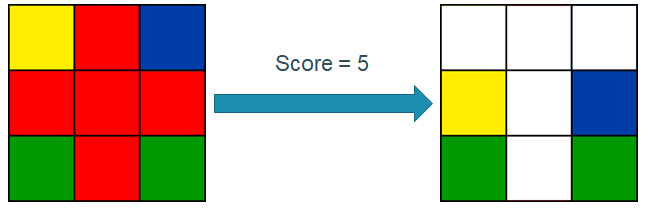
\includegraphics[height=18truemm]{game_score}
  \caption{Stel dat de blok in figuur~\ref{fig:game_change_blocks} rood werd, dan staan er 3 blokken met dezelfde kleur naast elkaar. Het spel verwijdert deze blokken en voor elke blok die verwijdert is krijgt de speler een punt. In dit geval heeft de speler 5 punten. De gele en de blauwe blok vallen naar beneden tot ze op een andere blok of op de bodem vallen.}
  \label{fig:game_score}
\end{figure}
\section{Modelleren}
\section{Evaluatiecriteria}

\chapter{Resultaten}
\chapter{Conclusie}

\newpage
% ----------------------- Achterblad ------------------------------
% Vergeet niet de tekst aan te passen:
% - Afdeling
% - Adres van de afdeling
% - Telefoon en faxnummer
% -----------------------------------------------------------------
\thispagestyle{empty}
\sffamily
%
\begin{textblock}{191}(113,-11)
{\color{blueline}\rule{160pt}{5.5pt}}
\end{textblock}
%
\begin{textblock}{191}(168,-11)
{\color{blueline}\rule{5.5pt}{59pt}}
\end{textblock}
%
\begin{textblock}{183}(-24,-11)
\textblockcolour{}
\flushright
\fontsize{7}{7.5}\selectfont
\textbf{Faculteit Computerwetenschappen}\\
Geel Huis, Kasteelpark Arenberg 11 bus 2100\\
3001 LEUVEN, BELGI\"{E}\\
tel. + 32 16 32 14 01\\
%fax + 32 16 00 00 00\\
www.kuleuven.be\\
\end{textblock}
%
\begin{textblock}{191}(154,-7)
\textblockcolour{}
\includegraphics*[height=16.5truemm]{sedes}
\end{textblock}
%
\begin{textblock}{191}(-20,235)
{\color{bluetitle}\rule{544pt}{55pt}}
\end{textblock}
\end{document}
